
Vi har nu en flade i $\mathbb{R}^3$ med parameterfremstillingen \\
$$\textbf{F}_{2}(x,y)=(x, y, \frac{1}{3}x^3), (x,y) \in \mathbb{R}^2 $$\\
Vi antager at vi på denne flade kan finde en geodæt  der svarer til en kurve (t, y(t)) i $\mathbb{R}^2$ \\
Vi antager at vi på denne flade kan finde en geodæt  der svarer til en kurve (t, y(t)) i $\mathbb{R}^2$ \\
Det første vi vil gøre er at finde udtrykket af længden på denne kurve samt opskrive dens Euler-Lagrange ligning. Mens vi gør dette vil vi også gerne finde dens orden og finde ud af om den er lineær. \\
Først opskriver vi vores funktion for vores kurve $(t,y(t), \frac{1}{3} t^3)$. Det næste vi gør er så at opskrive vores Lagrange funktion som vi finder ved at tage det bestemte integrale fra a til b for kvadratroden af vores differentierede funktion sat i anden. I dette tilfælde giver dette os denne funktion \\
$$L=\int_{a}^{b} \sqrt{1^2+ \dot{y}(t)^2+t^4}dt. $$\\
Denne Lagrange funktion sætter vi så ind i vores Euler-Lagrange ligning $ \frac{ \partial L}{ \partial y}-  \frac{d}{dt} \frac{ \partial L}{ \partial \dot{y}}=0$ da der i vores Lagrange funktion ikke er noget y led kommer vores Euler-Lagrange ligning derfor til at se sådan her ud $ \frac{d}{dt} \frac{ \partial L}{ \partial \dot{y}}=0 $\\
Vi vælger nu at udregne denne ligning så det er lidt nemmere at se hvad der egentlig står i den. \\
$$ \frac{d}{dt} \frac{ \dot{y}(t)}{ \sqrt{1^2+ \dot{y}(t)^2+t^4}}=0  $$\\
$$ \frac{ \ddot{y}(t)+ \ddot{y}(t)t^4-2 \dot{y}(t)t^3}{\sqrt{1^2+ \dot{y}(t)^2+t^4}}=0 $$\\
Vi kan med dette se af vores differential ligning er af 2. orden og at den ikke er lineær. \\
Nu vælger vi så at løse vores Euler-Lagrange ligning med bestemte værdier y(0)=10 og y(2)=11 \\
Vi vælger her at bruge maples dsolve kommando til at finde vores funktion som kommer til at se ud på følgende måde \\
$$y(t)=10+ \frac{\int_{0}^{t}\sqrt{1+_zI^4}d_zI}{\int_{0}^{2}\sqrt{1+_zI^4}d_zI} $$ \\
Denne funktion vil vi gerne sammenligne med funktionen for den rette linje mellem disse to punkter \\
$$p(t)=10+ \frac{1}{2}t $$ \\
\begin{figure}
  \caption{Den rette linje (nederst) og vores geodæt (øverst)}
  \centering
    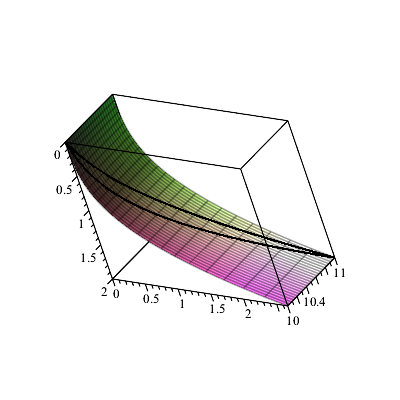
\includegraphics[scale=0.4]{thomas_graf}
\end{figure} \\
For at gøre dette vil vi gerne finde længden af de to for at se om vores funktion faktisk også er en geodæt på fladen mellem de to punkter. Vi starter med at finde længden af vores funktion. \\
$$ \frac{d}{dt} \frac{10+\int_{0}^{t}\sqrt{1+_zI^4}d_zI}{10+\int_{0}^{2}\sqrt{1+_zI^4}d_zI}$$ \\
$$ \int_{0}^{2}\sqrt{1^2+ \frac{1+t^4}{\int_{0}^{2}\sqrt{1+_zI^4}d_zI}^2+t^4}dt=3,79  $$\\
Vi gør herefter det samme for den rette linje \\
$$ \frac{d}{dt}10+ \frac{1}{2}t $$\\
$$\int_{0}^{2}\sqrt{1^2+\frac{1}{2}^2+t^4}dt=3,82 $$\\
Vi kan hermed se at lægnden af vores funktion er kortere end længden af funktionen med den rette linje.
